\hypertarget{link_to_tf2p2z}{}{\Large \bf tf2p2z}

{\it Transfer function between input and output: two real zeros and two real poles}

\begin{center}
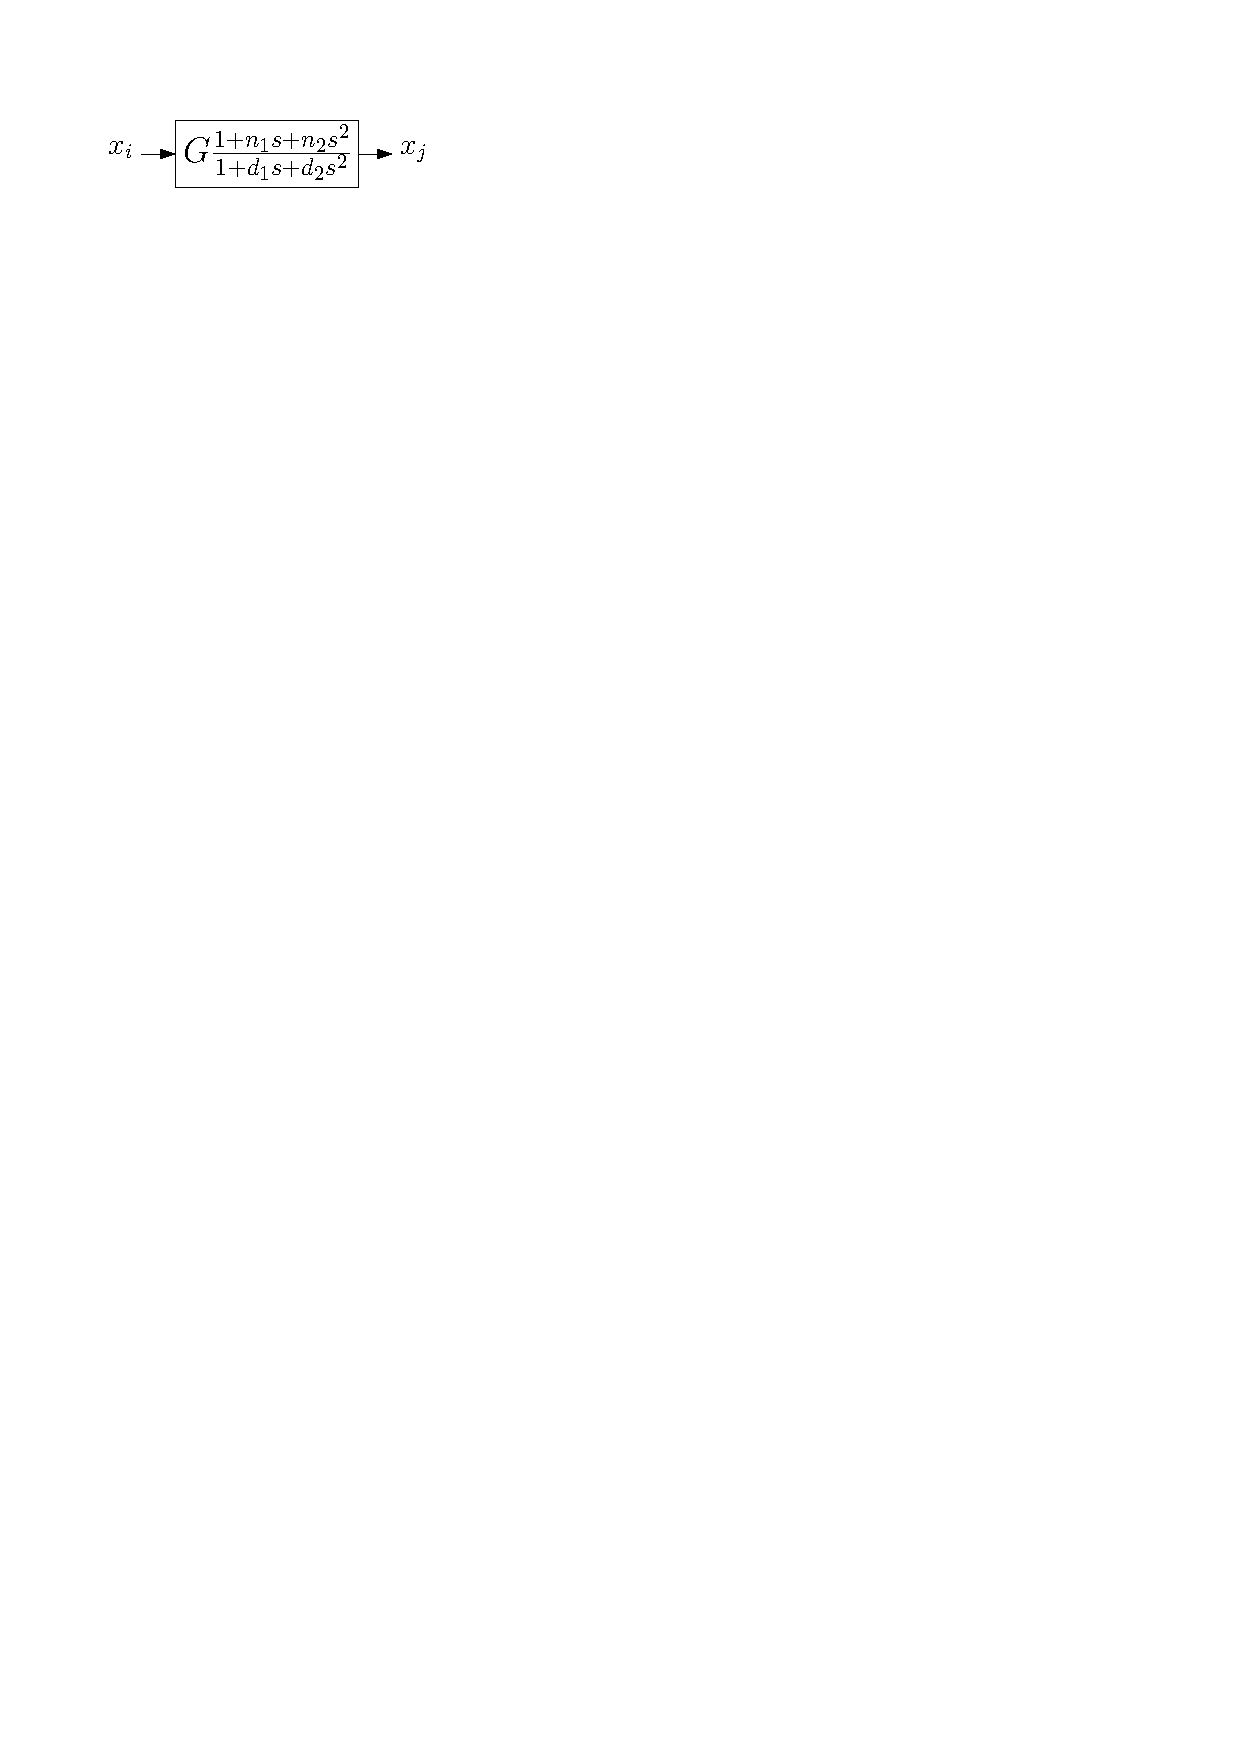
\includegraphics{codegen/tf2p2z.pdf}
\end{center}

Syntax : \hspace*{10ex}\parbox[t]{\textwidth}{\sf 
\& tf2p2z\\
name of variable $x_i$\\
name of variable $x_j$\\
data name, parameter name or math expression for $G$\\
data name, parameter name or math expression for $n_1$\\
data name, parameter name or math expression for $n_2$\\
data name, parameter name or math expression for $d_1$\\
data name, parameter name or math expression for $d_2$
}

~ \hrule ~

Internal states : $x_1$ ~~ and ~~ $x_2$

Discrete variables : none

\setcounter{equation}{0}

Equations : correspond to a second-order state space model with controllable canonical form:
\begin{eqnarray}
\dot{x_1} & = & x_2 \label{tf2p2z-1} \\
d_2 \: \dot{x_2} & = & - x_1 - d_1 x_2 + d_2 x_i \label{tf2p2z-2} \\
0 & = & G (d_2 - n_2) x_1 + G (n_1 d_2 - d_1 n_2) x_2 + G n_2 d_2 x_i - d_2^2 x_j \label{tf2p2z-3}
\end{eqnarray}

Initialization of internal states :  ~ $x_2=0$ ~~ and ~~ $x_1=d_2 x_i$

\vspace{2ex}
{\bf Exception}. If a small value is specified for $d_2$, namely if $d_2<0.005$, both $d_2$ and $n_2$ are set to zero and the transfer function becomes:
\[ G \frac{1 + n_1 s}{1+ d_1 s} \]
as considered in the {\tt tf1p1z} block.

If, in addition, a small value is specified for $d_1$, namely if $d_1<0.005$, both $d_1$ and $n_1$ are set to zero and the block behaves as a simple gain:
\[ x_j = G x_i \]